\chapter{Advantages and disadvantages}
Since in the previous chapters the majority of advantages and disadvantages of the protocol have been already discussed, in this chapter we complete our \textit{\oauth} description by showing a complete work flow comparison (taking into account other flows defined by the protocol but not so used nowadays) and a brief introduction on the extensions in order to better understand its peculiarities. 

\minitoc
\section{Secondary flows comparison}
Until now, all the practical aspects of the standard \rfc{6749} \cite{RFC6749} have been analyzed, but not all the defined ones. In particular, there are two other types of work flows in the specification: \textit{Resource Owner Password Credentials Grant} and \textit{Client Credentials Grant}. These two flows are not frequently used, but they can be helpful in some particular cases.

\subsection{Resource Owner Password Credentials Grant}
Described in Section 4.3 of the specification, this flow operates by using the user's actual credentials to gain an access token. It is not the best in terms of security. This goes against the other grant types, where the client application is completely unaware of the user's credentials. However, in this grant type, users send their credentials to the client application that, on their behalf, uses those credentials to access protected resources.
Once the client application has a user's credentials, it uses them to gain an access token, just as in the other grant types. In this sense, risk is slightly mitigated, compared to using the credentials directly, since tokens have limited scope and duration (unlike passwords). However, the passing and delegation of user credentials is highly undesirable due to the risk of leaking this important information.

Nevertheless, it could be useful when neither of the two others flows are available (implicit grant and authorization code grant).

\subsection{Client Credentials Grant}
Described in Section 4.4 of the \rfc{6749}, this type of flow is slightly different from the others. While the first three of them request access tokens on behalf of a user, this last one request access tokens on behalf of the client application. There may be occasions where the client application has resources with a service provider that are owned and consumed by the client application itself, and not by an end-user. For instance, a client application that uses Amazon RDS\footnote{Amazon Relational Database Service, "[...] makes it easy to set up, operate, and scale a relational database in the cloud. It provides cost-efficient and resizable capacity while automating time-consuming administration tasks such as hardware provisioning [..]". Source: \url{https://aws.amazon.com/rds/}} to persist its own application data (as opposed to a user's data). In this case, this grant is preferred. With this workflow, the client application can request an access token on its own behalf and then use that access token to access the protected resources it needs. The good news are that no user intervention is required and no additional risk is exposed.

\section{\oauth\ extensions}
Extensions are an ample, sophisticated and important key concept of the \oauth\ protocol. Indeed, they do not fall into the same specification and more or less everyone of them has its own RFC.

The implicit and the authorization code grant flows represent the majority of flows that application developers use. However, it is only a limited view with respect to the larger range of capabilities allowed by the framework. There are many extensions that can be added to the Open Authorization Framework to facilitate many additional use cases, but surely the most important ones are \textit{token types}, \textit{custom grant types} and \textit{OpenID Connect}.

\subsection{Token types}
Once a grant type is decided, the client application will interact with a service provider through the exchange of tokens. Once the user authenticates and authorizes the application, they are given a bearer token [\rfc{6750}], which the application can then use to access a protected resource on his behalf. The properties of these tokens are quite loosely defined, described by the specification simply as opaque string values that encapsulate an authentication for a particular user. They can simply be unique strings that match up with a set of permissions for a user. Many service providers implement their tokens in this non-standard, custom way. However, it is useful to know that there are two popular token formats that can be used by service providers, if desired:

\begin{itemize}
    \item JSON Web Tokens (JWT), described in \rfc{7519} \cite{RFC7519}
    \item SAML assertions, described in \rfc{7522}
\end{itemize}

Both of these token formats describe a standard for the creation and usage of security tokens. These tokens are known as security tokens, because they make use of cryptography to facilitate features that would not normally be allowed via simple opaque string values.

JWTs are most commonly seen in the consumer space (they are used in the OpenID Connect protocol). Compared with SAML assertions, JWTs can be considered a simpler version of security token than a SAML assertion, with a simpler format and encoding syntax. SAML assertions, on the other hand, employ a standard for security tokens that is more expressive and powerful than JWTs, at the expense of added complexity. These will typically be seen in the enterprise space where SAML integration for authentication is more prevalent. Both of these formats can act as bearer tokens in the \oauth\ protocol, as long as they are supported by the service provider.


\subsection{Custom grant types}
When the client application interacts with a service provider, such as Facebook, it does so by using a particular, predefined grant type. Previously, they have been discussed the two most commonly used grant types:

\begin{itemize}
    \item Authorization code grant
    \item Implicit grant
\end{itemize}

\noindent And the two additional grant types that are supported:

\begin{itemize}
    \item Resource owner password credentials grant
    \item Client credentials grant
\end{itemize}

\noindent They, as it has already been explained, are less commonly supported by consumer service providers, such as Google and Facebook. However, it must be pointed out that in addition to natively supporting these four grant types, the \textit{\oauth} framework allows for the specification of additional custom grant types. These will be determined and implemented by the service provider. So, perhaps a workplace decides to use \textit{\oauth} to restrict access to certain parts of the company's data, but the IT team and security team do not want to use any of the four natively supported grant flows. They can, instead, design and implement their own grant type, which the client application will subsequently use to request access tokens and access those protected resources.

\subsection{Authorization backend}
One of the major benefits of the \oauth\ protocol is that it has the ability to encapsulate and abstract away the authentication layer of a service, wrapping it with a standard, uniform layer for client applications to consume. For instance, a company may be using a Kerberos-based authentication system (e.g. LDAP [\rfc{4511}]), for the company's internal authentication. They may, at some point, choose to wrap this with an \oauth\ layer, which would effectively encapsulate their authentication layer and present a uniform interface to any interested parties. Now, they can change their internal authentication methodologies, say, to SAML, and clients would be largely unaware of that (they may be presented a different user consent screen, but other than that, behavior should be unaffected). This is a very powerful concept. Abstracting away the authentication layer provides a uniform interface for clients while maintaining flexibility for the underlying protocols to change without affecting (that is, breaking) clients.

\subsubsection{OpenID Connect}
The framework describes a protocol for managing authorization to protected resources for a service. It does not, however, describe methods for authentication. \textit{OpenID Connect} \cite{openid} is a protocol built on top of \textit{\oauth} in order to provide a complete solution for both authentication and authorization. As showed in Fig.~\ref{fig:oidc}, OIDC provides an identity layer on top of the authorization protocol described by \oauth. It allows clients to check the identity of an end-user when it authenticates in order to  authorize the \oauth\ consent. Most importantly, this can all be done by the client application without having to store or manage passwords.

\begin{figure}
    \centering
    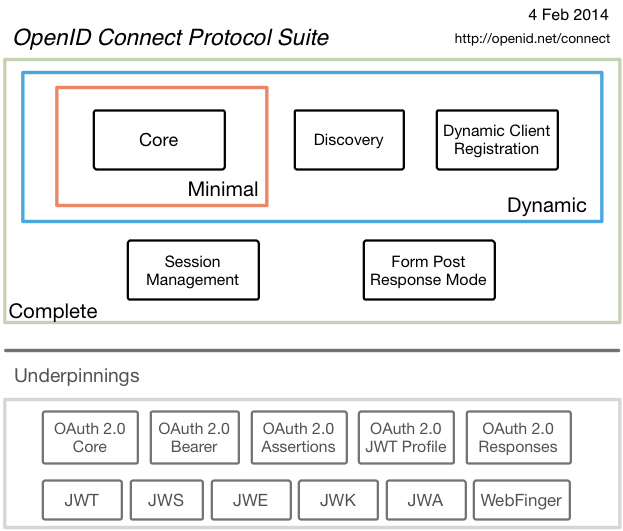
\includegraphics[scale=2.0]{chapters/images/chp3/OpenIDC-map.png}
    \caption[OpenID Connect protocol suite]{OpenID Connect protocol suite\\\hspace{\textwidth}Source:\hspace{0.2cm}\url{https://openid.net/connect/}}
    \label{fig:oidc}
\end{figure}

Previously, the concepts of \textbf{federated identity} and \textbf{delegated authority} have been introduced and it has been mentioned that they are actually the same underlying concept. In one delegated authority scenario, the user delegates authority for a client application to access some protected resource on their behalf, say, access to their Facebook friend list. However, this protected resource could be anything. It could even be their profile information as stored by Facebook. Delegating access to this resource gives the client application the means of verifying the end-user's identity without ever seeing their credentials. As an example, it is interesting how this is accomplished with OpenID Connect using a familiar \oauth\ workflow. What follows is a modified version of the authorization code grant flow that we explored previously:

\begin{itemize}
    \item[1.] The client application initiates the authorization request using the authorization code grant flow. However, in this authorization request, a subset of the following OpenID Connect scopes is requested:
    \item[] \begin{itemize}
        \item \texttt{openid}: REQUIRED. It means that the client is making an OIDC request
        \item \texttt{profile}: OPTIONAL. This requests access to the user's
    profile information
        \item \texttt{email}: OPTIONAL. This requests access to the user's e-mail address
        \item \texttt{address}: OPTIONAL. This requests access to the user's  address information
        \item \texttt{phone}: OPTIONAL. This requests access to the user's phone number
    \end{itemize}
    
    \item[2.] Here the server must validate the parameters. In particular, OIDC defines more OPTIONAL params (e.g. \texttt{nonce}, \texttt{prompt} and so on) that are essential to manage the authentication (e.g. rather than the authentication itself, whether the user is already authenticated or not). After that the server validates the parameters, if it is a valid request for login, the user is presented with the same user consent screen that we are familiar with, with the difference that it MAY be specified that the user authorizes the relying party (client) to authenticate it. If it accepts, it will be redirected back to the client application via the redirection endpoint, passing along with it the corresponding authorization code (as \oauth\ requires).
    \item[3.] The client application will take this authorization code and make a request to the service provider's token endpoint to exchange it for an access token. The server must know that the corresponding AuthZ code was issued from a OIDC authentication request and must check the client\_id correspondence of it. It builds up the \texttt{id\_token} that is a JWT which contains private claims about the authenticated user (\texttt{name}, \texttt{address} and so on) and other claims defined in the Section 4.1 of the \rfc{7519} \cite{RFC7519} (such as \texttt{iss} that represents the issuer and \texttt{sub} that represents a unique identifier of the authenticated user).
    \item[4.] The response from this request will contain an access token (as the property \texttt{access\_token}). However, it will contain the additional token known as an \textit{ID token} (as the property \texttt{id\_token}). The client MUST decrypt the token by using the specified cryptographic operations contained in the JOSE Header (Section 5 of \rfc{7519}), validate the JWT ID Token and retrieve the claims about the user, the issuer and so on, in order to ensure the truthfulness of the message response. Finally, the user identity provided by the AuthZ server using OIDC on top of \oauth\ is verified.
\end{itemize}


As it can be seen, this flow is very similar to the authorization code grant flow that has been discussed earlier, except now it is possible to verify the identity of the user by consuming the ID token built and signed by the AuthZ server, something that was not possible to do with \oauth\ alone. It is an elegant solution for providing a full end-to-end authentication and authorization framework.